\subsection{Normal Use}
We consider normal use the main feature of the system, meaning making a reservation for a service.\\
This is achieved by the user starting a search for the service they wish to use and if at least one result is found the list is displayed to the customer that will then select the one he/she wishes to reserve.
\begin{figure}[!htb]
\centering
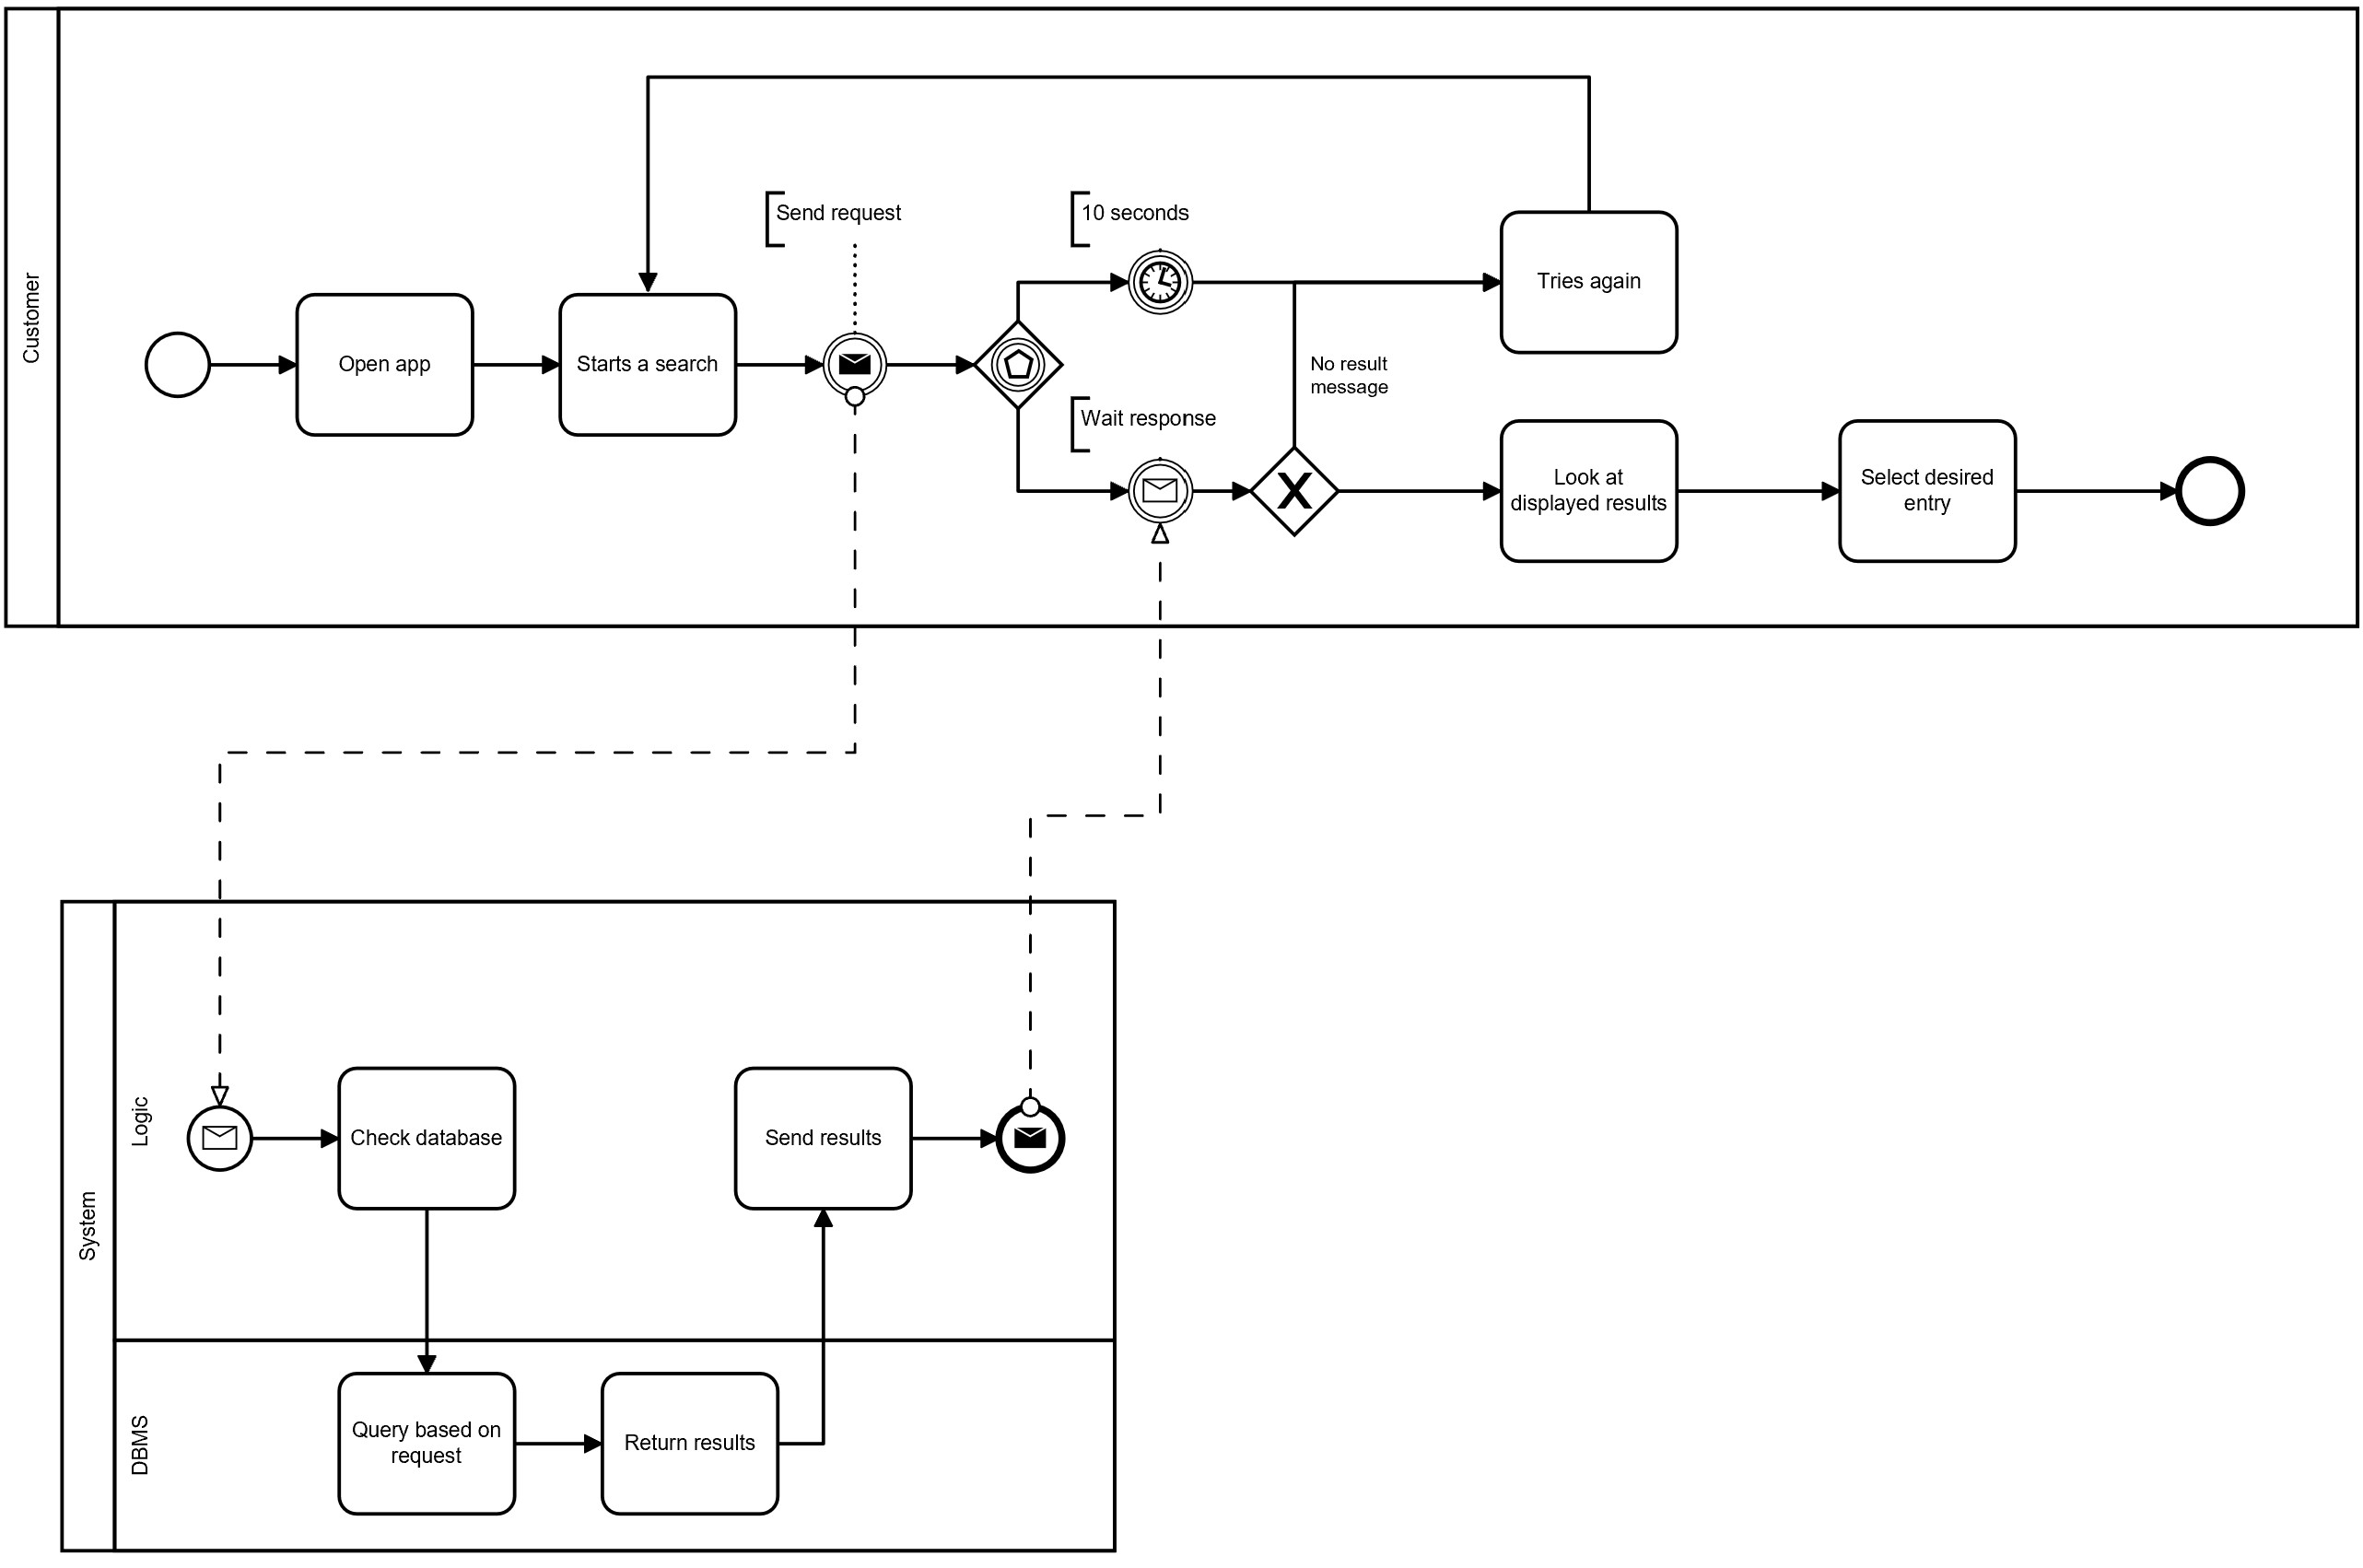
\includegraphics[width=1.0\textwidth, angle = 90]{Img/DiagramNormalUse.jpg}
\caption{Ordinary application use diagram}
\end{figure}
\clearpage
\subsection{Inserting a Review}
When inserting a review a customer needs to open the application and write one, then if the back-end system accepts it, it will be stored in the database for other customers to see (N.B. in the implementation we opted for a simpler stars system, meaning that there is not an actual "writing" and unless data is corrupted or a connection is missing no method of rejecting the review is in place).
\begin{figure}[!htb]
\centering
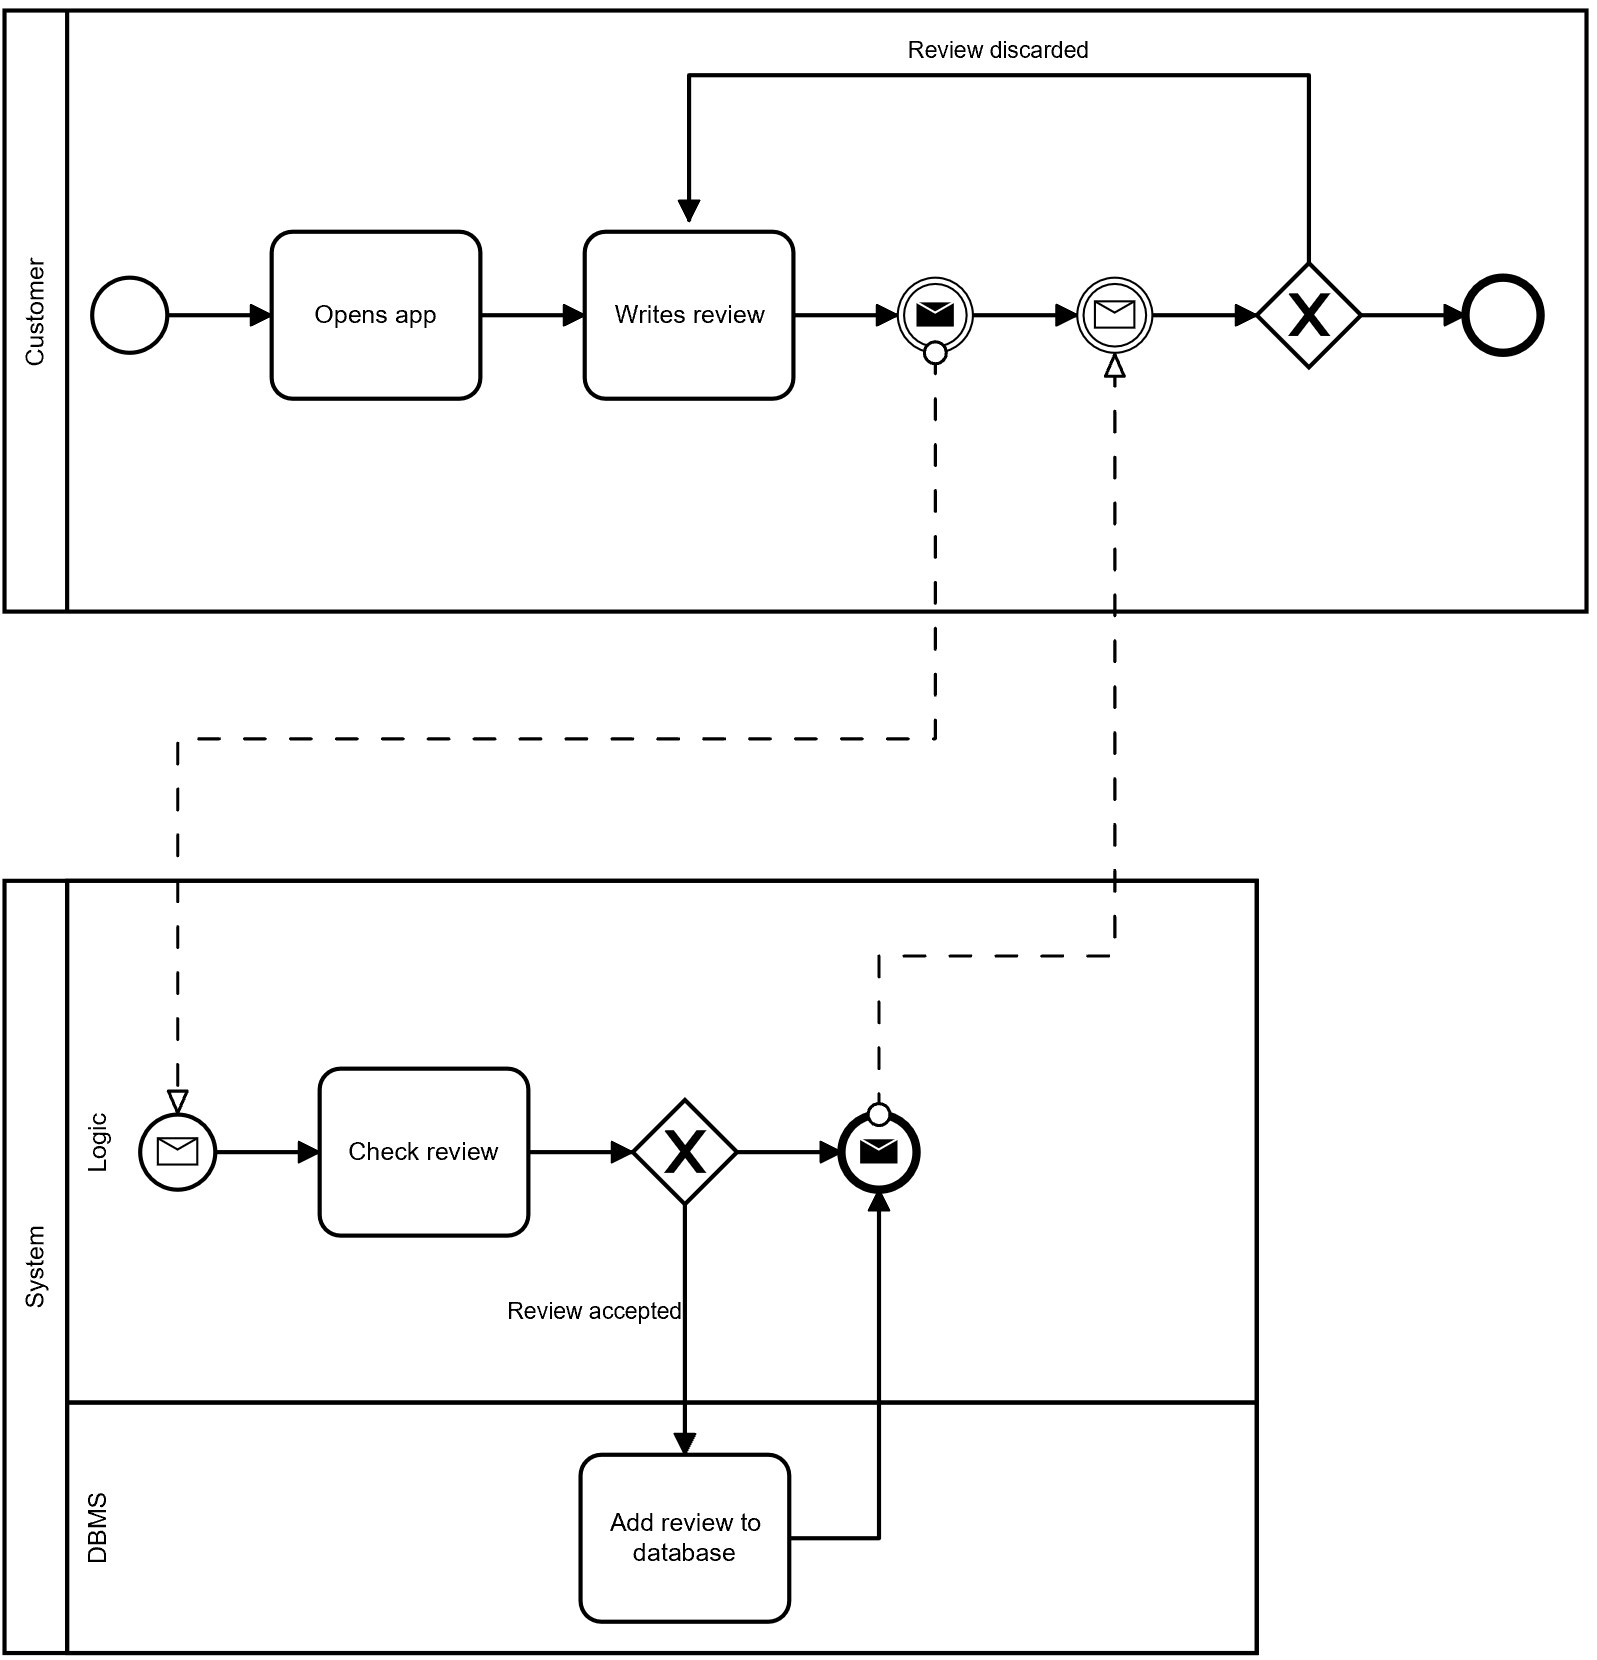
\includegraphics[width=1.0\textwidth]{Img/DiagramReview.jpg}
\caption{Review making diagram}
\end{figure}
\clearpage
\subsection{Payment}
We also considered the possibility of a payment system inside the application during development, but ultimately decided not to include it in the prototype as there would be no need for it for demonstration purposes since it would relay almost entirely on external tools/APIs (i.e. PayPal).\\
A brief diagram is shown below anyways, highlighting how the user needs only to send a payment request and wait for a response, much like our system itself that will only act as "bridge" between the user and the black box that it is the service by forwarding messages to one another.
\begin{figure}[!htb]
\centering
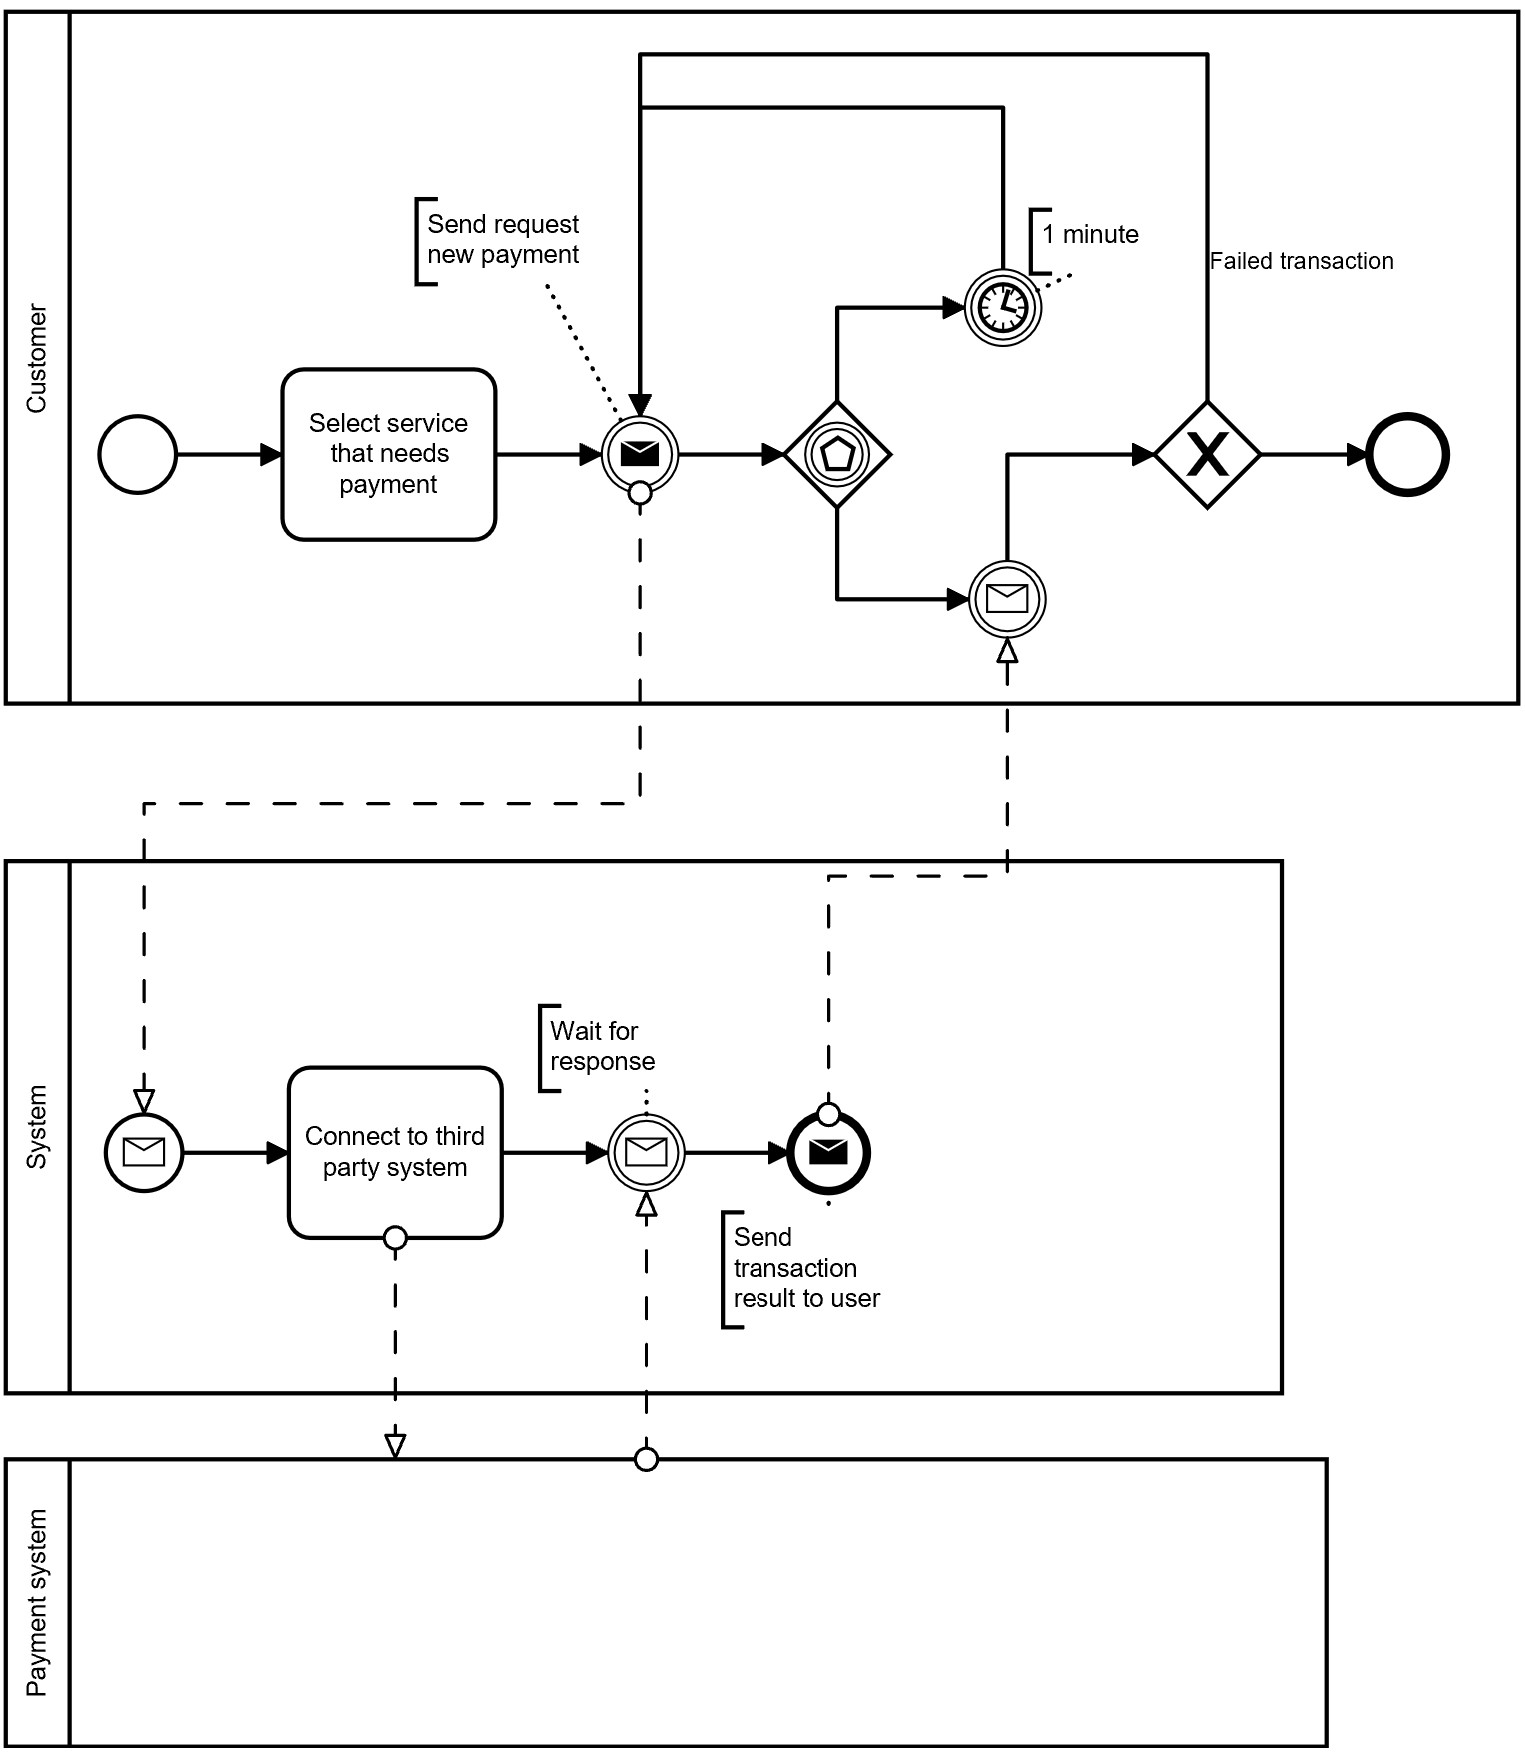
\includegraphics[width=1.0\textwidth]{Img/DiagramPayment.jpg}
\caption{Payment execution diagram}
\end{figure}
